\section{ZooScan扫描仪}

ZooScan扫描仪完成的任务:
\begin{itemize}
\item 扫描空白背景
\item 扫描样品,获得原始图片和元数据信息
\end{itemize}

\subsection{操作步骤}
\subsubsection{创建项目}
\begin{itemize}
\item 打开``Image J'',在软件界面中,选择项目选项表最后的 ``CREATE NEW PROJECT'',创建一个新的项目。如图~\ref{fig:create}。
    \begin{figure}[!ht]
    \centering
    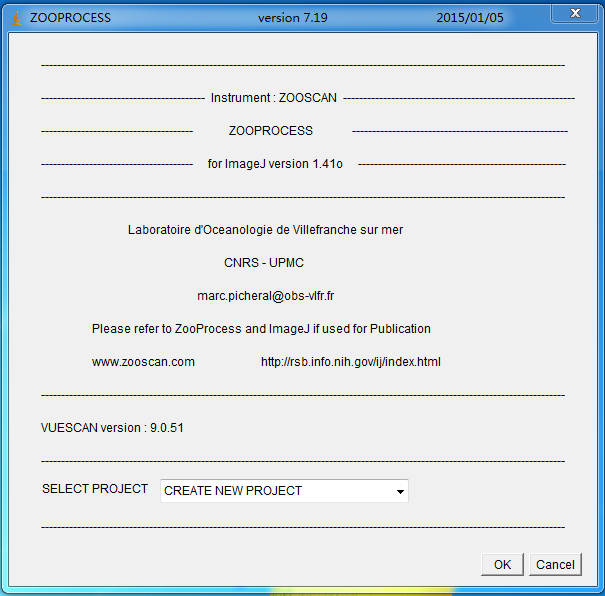
\includegraphics[width=3in]{create}
    \caption{创建项目}
    \label{fig:create}
    \end{figure}
\item 选择扫描选项。选择2400dpi分辨率和``Large''的扫描框(15$cm$ $\times$ 24$cm$)。如图~\ref{fig:frame}。
    \begin{figure}[!ht]
    \centering
    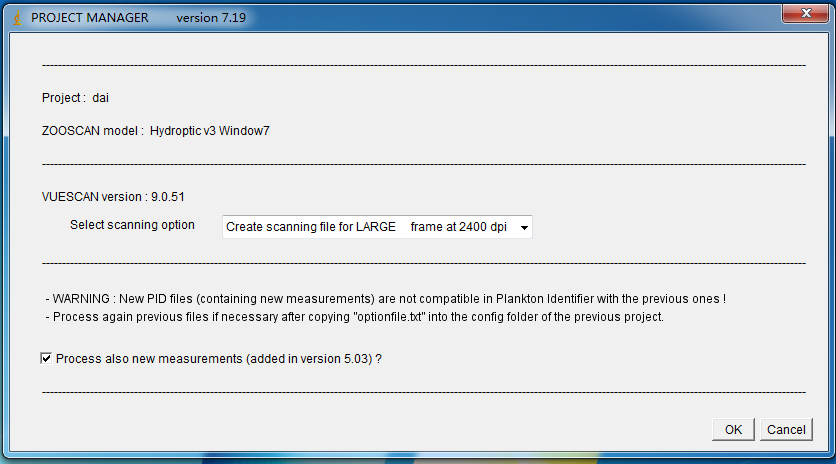
\includegraphics[width=3.5in]{frame}
    \caption{选择分辨率和扫描框大小}
    \label{fig:frame}
    \end{figure}
\item 输入样品的元数据(metadata)。在后面处理过程中,可以通过ZooProcess中的\textbf{``EDIT and MODIFY metadata''}工具来修改元数据。如图~\ref{fig:metadata}。
    \begin{figure}[!ht]
    \centering
    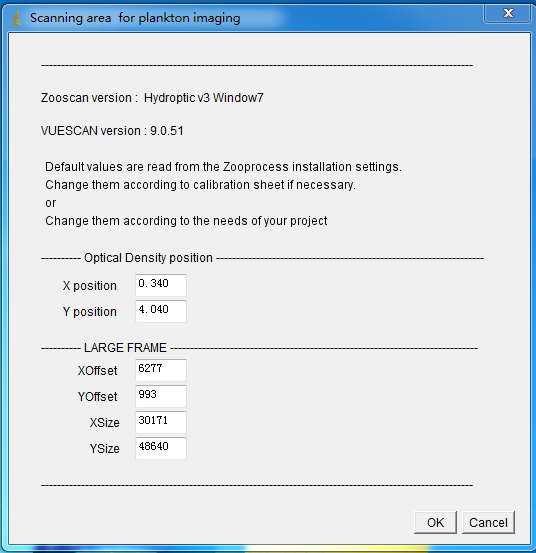
\includegraphics[width=3.0in]{metadata}
    \caption{输入扫描信息}
    \label{fig:metadata}
    \end{figure}
\end{itemize}


\subsubsection{扫描背景}
背景图像是一张空白图像,用于图像分析过程中。在与样品相同环境下 (自来水或是过滤海水),先扫描背景再扫描样品。最好是在每个扫描任务开始时,都扫描一次背景图像。
\begin{itemize}
\item 用清水清洁和冲洗ZooScan托盘和表面玻璃,时不时地检查并清除在玻璃和扫描框上的污点。
\item 倒一些清水(保持在室温)没过托盘,它可以防止扫描框刮擦托盘。
\item 放置扫描框(15$cm$ $\times$ 24$cm$),这取决于之前ZooProcess中的``创建项目''中的选项。
\item 在预扫描和实际扫描之间,等待30秒。
\end{itemize}

\subsubsection{准备样品}
\begin{itemize}
\item 存储几升清水,保持在室温,用来为ZooScan注水。
\item 用筛子(网格间隙为100$\mu m$ )过滤掉防腐剂和海水中物质。样品通过间隙为1$mm$和200$\mu m$的两种网格,将浮游生物分成不同体型的两部分。
%%\item 用木棒将粘连的浮游生物分离开,且避免浮游生物贴靠扫描框边缘。
\item 浮游生物被分为不同体型的两部分:一个为体型大的样品,另一个为体型小的样品。分别将分开后的样品,添加标签$d1$和$d2$,用于扫描后的数据处理过程中。如图~\ref{fig:volume}。
  \begin{figure}[!ht]
  \centering
   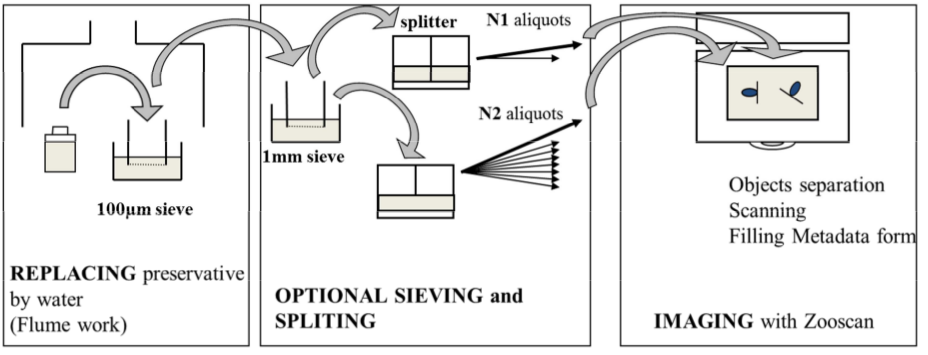
\includegraphics[width=3.6in]{volume}
    \caption{准备样品}
    \label{fig:volume}
   \end{figure}
\item 使上述两个分开后的样品中,保持只有1000 $ - $ 1500个浮游生物。
\end{itemize}

\subsubsection{扫描样品}
\begin{itemize}
\item 在扫描托盘中加入量水,放置扫描框(15$cm$ $\times$ 24$cm$),调整扫描框放置的位置(位置在扫描托盘中有标注)。
\item 倒入样品,加入清水,直到没过扫描框的台阶。
\item 将个体较大的浮游生物放在扫描框的中心,用木棒分离粘连浮游生物,避免浮游生物贴靠扫描框边缘。对于漂浮在水面的浮游生物,轻轻用木棒将浮游生物压入水中。如果存在无法没入水中的浮游动物,且数量不多,则将它们移出 ({\color{blue} 这一步是生成好的数据质量的关键步骤})。如图~\ref{fig:sticks}。
  \begin{figure}[!ht]
  \centering
   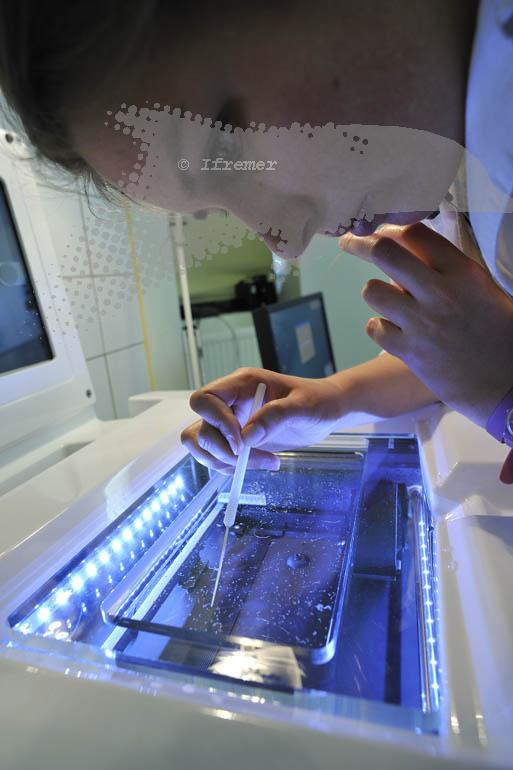
\includegraphics[width=2.0in]{sticks}
    \caption{用木棒分离粘连浮游生物}
    \label{fig:sticks}
   \end{figure}
\item 检查托盘是否有气泡,顶盖玻璃的表面是否冷凝。
\item 加载ZooProcess,选择项目,点击扫描样品,选择两部分样品中的一个样品($d1$和$d2$),写入相关元数据。
\end{itemize}

\subsubsection{回收样品}
\begin{itemize}
\item 清洁托盘,避免下次实验污染了样品。
\item 移走并冲洗透明的扫描框,回收所有的标本。
\item 清洁干燥扫描托盘。
\end{itemize}


\subsection{注意事项}
\begin{itemize}
\item 清水可以是自来水或过滤海水,保持在室温是为了避免在ZooScan的托盘中产生气泡或者顶盖玻璃上出现冷凝。因为自来水管中的自来水和房间的温度存在一定温差。
\item ZooScan提供1200dpi和2400dpi两种分辨率扫描。分辨率限制在2400dpi,是由于ZooScan设计的光路需要空气入水和由水进入玻璃两次穿过界面,使成像分辨率收到限制。
\item ZooScan的扫描框有两个尺寸:11$cm$ $\times$ 24$cm$ 和 15$cm$ $\times$ 24$cm$。推荐使用15$cm$ $\times$ 24$cm$的扫描框,具体使用哪个扫描框由ZooProcess中的选项决定。
\item 扫描空白背景不仅可以去除灯光产生的异质性的斑点等,而且可以检验系统的稳定性。
%%\item 防止大个且数量较少的浮游生物被低估
\item 在准备样品阶段,通常情况下,将样品分为两个或以上的小样品进行扫描。
\item 在准备样品阶段,如何将浮游生物样品分成不同的小样品,取决于原样品中浮游生物的种类多少与体型大小。
\item 扫描的浮游生物必须保持不动的状态,使用固定剂或将其麻醉。
\item 扫描框上有5mm的小台阶,注入的水必须漫过这台阶的高度,避免在扫描后的图像边缘出现弯液面现象。如图~\ref{fig:step}。
  \begin{figure}[!ht]
  \centering
   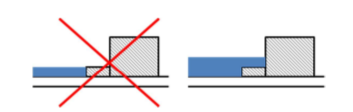
\includegraphics[width=2.8in]{step.png}
    \caption{框的台阶高度}
    \label{fig:step}
   \end{figure}
\item 在较大的框内(15$cm$ $\times$ 24$cm$),最多可以容纳1000 $ - $ 1500个浮游生物。
\item 在ZooProcess中也可以对扫描图像中的粘连浮游生物进行分离,但是最好是在样品扫描之前用木棒进行分离。如图~\ref{fig:separate}。
  \begin{figure}[!ht]
  \centering
   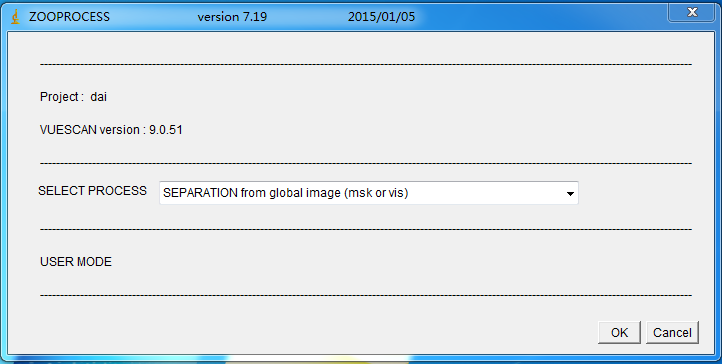
\includegraphics[width=3.5in]{separate}
    \caption{ZooProcess的浮游生物分离}
    \label{fig:separate}
   \end{figure}
\end{itemize}
